\documentclass[dvipsnames]{AritzhClass}

\usepackage{array}

\izenburua{Nonograma}
\azpiizenburua{Proiektuaren Txostena}
\smalltitle{Nonograma: Txostena}
\ikasgaia{Ingeniaritza Informatikoa: KE}
\author{Iñigo Arnedo eta Ane Odriozola}
\data{\today}

\begin{document}

\izenburuorrialdea

\tableofcontents

\pagebreak

\section{Proiektuaren enuntziatua}

Nintendo DS-rako \textit{100 doors} jokuaren motako ate bat diseinatu eta programatu, DS-aren pantaila, teklatua eta denboragailua erabiliz.

\section{Proiektuaren definizioa: Nonograma}

Nonograma adimen joko japoniar bat da, Sudoku baten antzekoa, baina kasu honetan ezker- eta goi-marginetan agertzen diren zenbakietan oinarrituz, laukiak bete behar dira, irudi bat lortzeko. Goi-marginan agertzen diren zenbakiak zutabe horretan laukiak nola bete behar diren adierazten dute. Zifra bakoitzak segidan dauden lauki beltz kopuru bat adierazten du. Hortaz, zutabe baten gainean \textit{$\left\langle\!\left\langle\, 5\, \right\rangle\!\right\rangle$} bat agertzen bada, zutabe horretan nonbait 5 lauki segidan daudela adierazten du; \textit{$\left\langle\!\!\!\left\langle\!\!\!\begin{array}{c}1 \\ 5\end{array}\!\!\!\right\rangle\!\!\!\right\rangle$} agertzen bada, aldiz, lauki bakar bat, eta gutxienez lauki txuri batengatik separatutako 3 lauki beltz agertzen direla adierazten du. Ezker-marginan dauden zenbakiekin berdina gertatzen da, baina hauek errenkada horretako lauki-konbinazioa adierazten dute.

\textit{100 doors} jokorako ate bat diseinatu behar genuenez, nonograma honetarako irudia giltza bat izatea adostu genuen, hauen bitartez irekitzen baitira ateak. 

\subsection{Jokoaren deskribapena}

Jokoa hasi orduko, pantailako lauki guztiak txuriz agertuko dira. Lauki txuri baten gainean behin sakatuz gero, beltz bihurtuko da, eta alderantziz ere, hau da, lauki beltz baten gainean sakatuz gero, txuri bilakatuko da. 

Jokoa errazteko asmoz, kontagailu bat gehitu diogu jokoari. Kontagailuak adieraziko du zenbat lauki aldatu behar diren (txuritik beltzera, zein beltzetik txurira) lortu behar den irudia, hots, giltza, lortzeko.

Hortaz, giltza 18 lauki beltzez osatuta dagoenez, hasieran kontagailuak 18 balioko du, eta giltzari dagokion lauki bat belztean, kontagailua dekrementatuko da; beste edozein laukiren kasuan, berriz, inkrementatuko da. Honela, erraz jakin daiteke belztutako karratu bat giltzaren parte den ala ez, kontagailuak jasan duen aldaketari erreparatuz, jokoa erraztuz. Gainera, modu honetan, kontagailuari bakarrik erreparatuz jakin daiteke jokoa irabazi den ala ez, izan ere, kontagailua 0 balioa hartuko du baldin eta soilik baldin giltza beterik badago.

Giltza bete denean, giltzaren gainean klikatu beharko da. Modu honetan giltza erabili izan denaren itxura emango du. 

\subsection{Adibideak}

\begin{taula}{}{argazkiTaula}{cc}
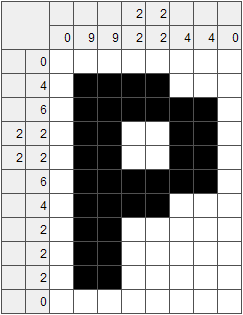
\includegraphics[scale=0.75]{nonograma1} & 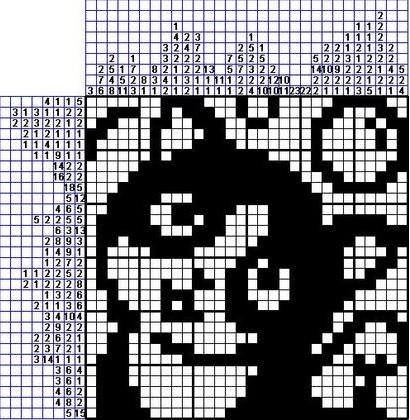
\includegraphics[scale=0.75]{nonograma2} \\
Adibide sinplea & Profesionalentzako bakarrik...
\end{taula}

\section{Automatak}
\subsection{Hasierako automata}
\begin{center}
\includegraphics[scale=0.4]{Nonograma_Mapa}
\end{center}
\subsection{Automataren hobekuntza}
\begin{center}
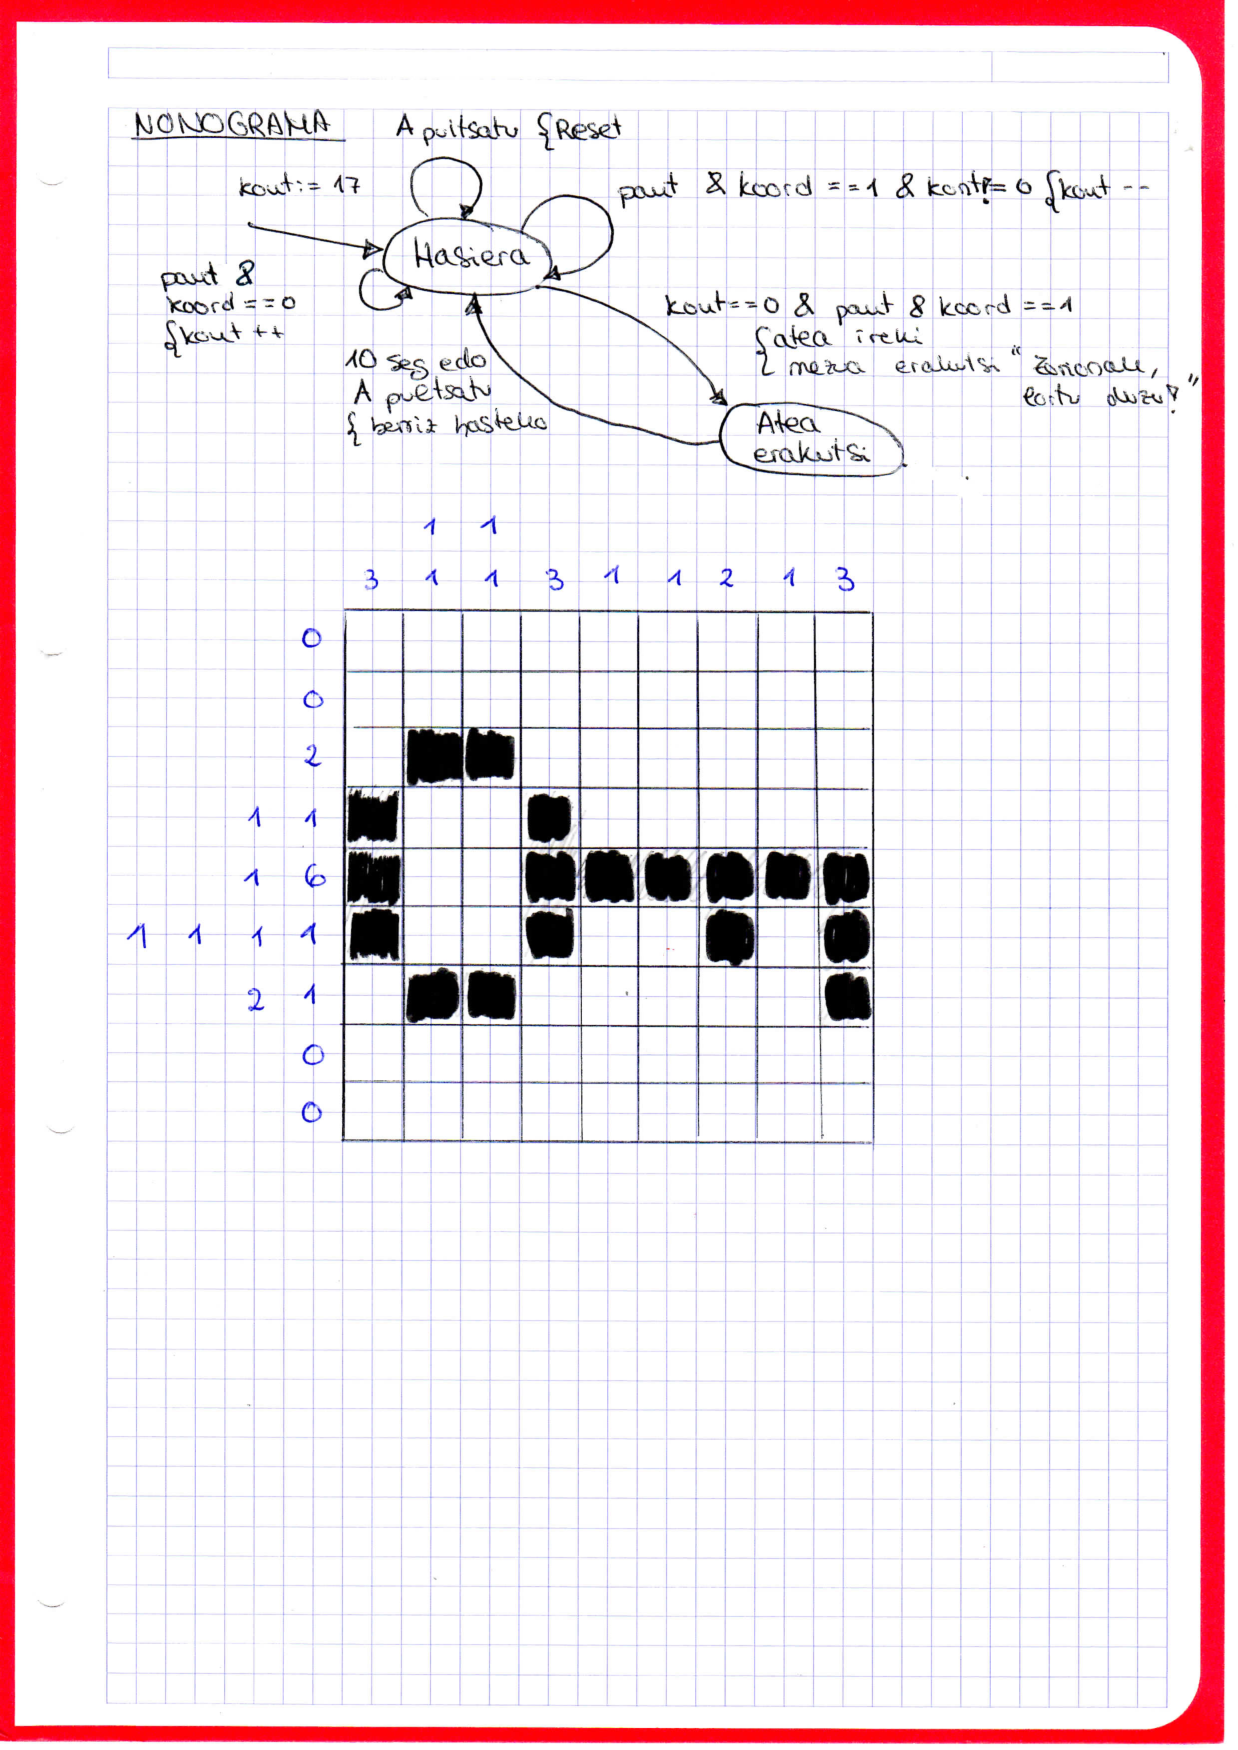
\includegraphics[scale=0.4]{img003}
\end{center}
\subsection{Behin-betiko automata}
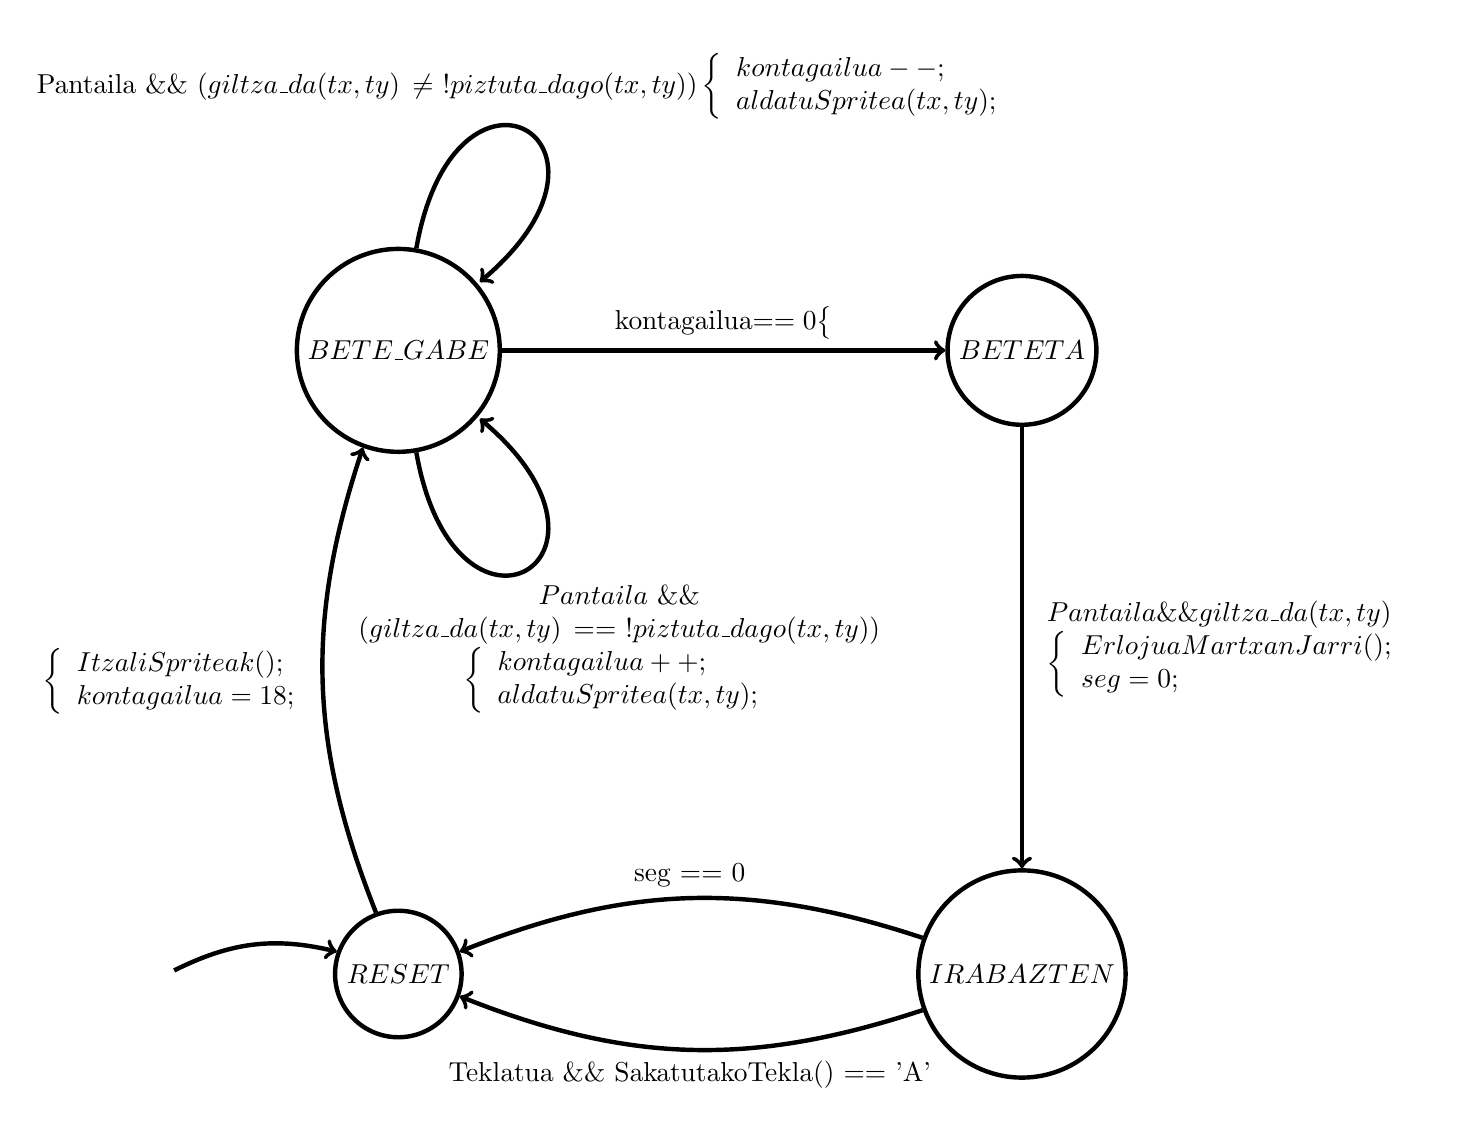
\begin{tikzpicture}[y=-1cm, scale=0.99, every node/.style={scale=0.99}]
\node(start) at (-3,8){};
\node(0) at (0,0)	[shape=circle,draw, ultra thick]	{$BETE\_GABE$};
\node(1) at (8,0)	[shape=circle,draw, ultra thick]	{$BETETA$};
\node(2) at (8,8)	[shape=circle,draw, ultra thick]	{$IRABAZTEN$};
\node(3) at (0,8)	[shape=circle,draw, ultra thick]	{$RESET$};
\path [ultra thick, ->]
  (start) edge [bend left=20] node [above] {} (3)
  (0) edge [in=40,out=80,loop] node [above] {Pantaila $\&\& \,\left(\text{giltza\_da}(tx, ty)\, \neq \,\, !\text{piztuta\_dago}(tx, ty)\right)\left\{\begin{array}{l}\text{kontagailua}--;\\ \text{aldatuSpritea(tx, ty);}\end{array}\right.$}
  (0) edge [in=320,out=280,loop] node [below right, xshift=-70] {$\begin{array}{c}\text{Pantaila} \,\, \&\& \\ \left(\text{giltza\_da}(tx, ty)\, == \,\, !\text{piztuta\_dago}(tx, ty)\right) \\ \left\{\begin{array}{l}\text{kontagailua}++;\\ \text{aldatuSpritea(tx, ty);}\end{array}\right.\end{array}$}
  (0) edge node [above] {kontagailua$==0 \big\{$} (1)
  (1) edge [below] node [right] {$\begin{array}{l}\text{Pantaila \&\& giltza\_da(tx, ty)} \\ \left\{\begin{array}{l}\text{ErlojuaMartxanJarri();}\\ \text{seg=0;}\end{array}\right.\end{array}$} (2)
  (2) edge [bend right=20] node [above] {seg == 0} (3)
  (2) edge [bend left=20] node [below] {Teklatua \&\& SakatutakoTekla() == 'A'} (3)
  (3) edge [bend left=20] node [left] {$\left\{\begin{array}{l}ItzaliSpriteak(); \\ kontagailua=18; \\ \end{array}\right.$} (0)
  ;
\end{tikzpicture}

\section{Nintendo DS-aren osagaien erabilpena}
\subsection{Denboragailua}
Behin jokoa amaituta, 10 segundu pasa eta gero \textit{A} tekla sakatzen ez bada jokoa berrabiarazi egingo da. 10 segundu horiek zenbatzeko erabili dugu denboragailua. Jokoa berrabiaraztean 10 segunduko kontagailu hori \textit{0}-ra itzultzen da eta berriz zenbatzen hasten da jokoa amaituz gero.
\subsection{Teklak}
\textit{A} tekla erabili dugu jokoa amaitzean tekla horren bitartez atea irekitzeko, nahiz eta ez den ikusten atea nola irekitzen den.
\subsection{Ukimen pantaila eta goiko pantaila}
Goiko pantaila jokoaren azalpenak bistaratzeko erabili dugu. Aldiz, ukimen pantaila jokatu ahal izateko erabili dugu. Ukimen pantailaren bitartez aukeratu behar dira laukitxoak irudia sortu ahal izateko. Horrez gain, ukimen pantailan ere laguntza ematen duten zenbakitxoak bistaratzeko ere erabili dugu. 
\end{document}
